%package list
\documentclass{article}
\usepackage[top=3cm, bottom=3cm, outer=3cm, inner=3cm]{geometry}
\usepackage{multicol}
\usepackage{graphicx}
\usepackage{url}
%\usepackage{cite}
\usepackage{hyperref}
\usepackage{array}
%\usepackage{multicol}
\newcolumntype{x}[1]{>{\centering\arraybackslash\hspace{0pt}}p{#1}}
\usepackage{natbib}
\usepackage{pdfpages}
\usepackage{multirow}
\usepackage[normalem]{ulem}
\useunder{\uline}{\ul}{}
\usepackage{svg}
\usepackage{xcolor}
\usepackage{listings}

\lstdefinestyle{ascii-tree}{
    literate={├}{|}1 {─}{--}1 {└}{+}1 
  }
\lstset{basicstyle=\ttfamily,
  showstringspaces=false,
  commentstyle=\color{red},
  keywordstyle=\color{blue}
}
%\usepackage{booktabs}
\usepackage{caption}
\usepackage{subcaption}
\usepackage{float}
\usepackage{array}

\newcolumntype{M}[1]{>{\centering\arraybackslash}m{#1}}
\newcolumntype{N}{@{}m{0pt}@{}}


%%%%%%%%%%%%%%%%%%%%%%%%%%%%%%%%%%%%%%%%%%%%%%%%%%%%%%%%%%%%%%%%%%%%%%%%%%%%
%%%%%%%%%%%%%%%%%%%%%%%%%%%%%%%%%%%%%%%%%%%%%%%%%%%%%%%%%%%%%%%%%%%%%%%%%%%%
\newcommand{\itemEmail}{jgordillome@unsa.edu.pe}
\newcommand{\itemStudent}{Jose Alonzo Gordillo Mendoza}
\newcommand{\itemCourse}{Programación Web 2}
\newcommand{\itemCourseCode}{20220577}
\newcommand{\itemSemester}{III}
\newcommand{\itemUniversity}{Universidad Nacional de San Agustín de Arequipa}
\newcommand{\itemFaculty}{Facultad de Ingeniería de Producción y Servicios}
\newcommand{\itemDepartment}{Departamento Académico de Ingeniería de Sistemas e Informática}
\newcommand{\itemSchool}{Escuela Profesional de Ingeniería de Sistemas}
\newcommand{\itemAcademic}{2023 - A}
\newcommand{\itemInput}{Del 14 Junio 2023}
\newcommand{\itemOutput}{Al 28 Junio 2023}
\newcommand{\itemPracticeNumber}{06}
\newcommand{\itemTheme}{Python - Django}
%%%%%%%%%%%%%%%%%%%%%%%%%%%%%%%%%%%%%%%%%%%%%%%%%%%%%%%%%%%%%%%%%%%%%%%%%%%%
%%%%%%%%%%%%%%%%%%%%%%%%%%%%%%%%%%%%%%%%%%%%%%%%%%%%%%%%%%%%%%%%%%%%%%%%%%%%

\usepackage[english,spanish]{babel}
\usepackage[utf8]{inputenc}
\AtBeginDocument{\selectlanguage{spanish}}
\renewcommand{\figurename}{Figura}
\renewcommand{\refname}{Referencias}
\renewcommand{\tablename}{Tabla} %esto no funciona cuando se usa babel
\AtBeginDocument{%
	\renewcommand\tablename{Tabla}
}

\usepackage{fancyhdr}
\pagestyle{fancy}
\fancyhf{}
\setlength{\headheight}{30pt}
\renewcommand{\headrulewidth}{1pt}
\renewcommand{\footrulewidth}{1pt}
\fancyhead[L]{\raisebox{-0.2\height}{
\includegraphics[width=3cm]{img/logo_episunsa.png}}}
\fancyhead[C]{\fontsize{7}{7}\selectfont	\itemUniversity \\ \itemFaculty \\ \itemDepartment \\ \itemSchool \\ \textbf{\itemCourse}}
\fancyhead[R]{\raisebox{-0.2\height}{
\includegraphics[width=1.2cm]{img/logo_abet}}}
\fancyfoot[L]{Estudiante Jose Gordillo Mendoza}
\fancyfoot[C]{\itemCourse}
\fancyfoot[R]{Página \thepage}

% para el codigo fuente
\usepackage{listings}
\usepackage{color, colortbl}
\definecolor{dkgreen}{rgb}{0,0.6,0}
\definecolor{gray}{rgb}{0.5,0.5,0.5}
\definecolor{mauve}{rgb}{0.58,0,0.82}
\definecolor{codebackground}{rgb}{0.95, 0.95, 0.92}
\definecolor{tablebackground}{rgb}{0.8, 0, 0}

\lstset{frame=tb,
	language=bash,
	aboveskip=3mm,
	belowskip=3mm,
	showstringspaces=false,
	columns=flexible,
	basicstyle={\small\ttfamily},
	numbers=none,
	numberstyle=\tiny\color{gray},
	keywordstyle=\color{blue},
	commentstyle=\color{dkgreen},
	stringstyle=\color{mauve},
	breaklines=true,
	breakatwhitespace=true,
	tabsize=3,
	backgroundcolor= \color{codebackground},
}

\begin{document}
	
	\vspace*{10px}
	
	\begin{center}	
		\fontsize{17}{17} \textbf{ Informe de Laboratorio \itemPracticeNumber}
	\end{center}
	\centerline{\textbf{\Large Tema: \itemTheme}}
	%\vspace*{0.5cm}	

	\begin{flushright}
		\begin{tabular}{|M{2.5cm}|N|}
			\hline 
			\rowcolor{tablebackground}
			\color{white} \textbf{Nota}  \\
			\hline 
			     \\[30pt]
			\hline 			
		\end{tabular}
	\end{flushright}	

	\begin{table}[H]
		\begin{tabular}{|x{4.7cm}|x{4.8cm}|x{4.8cm}|}
			\hline 
			\rowcolor{tablebackground}
			\color{white} \textbf{Estudiante} & \color{white}\textbf{Escuela}  & \color{white}\textbf{Asignatura}   \\
			\hline 
			{\itemStudent \par \itemEmail} & \itemSchool & {\itemCourse \par Semestre: \itemSemester \par Código: \itemCourseCode}     \\
			\hline 			
		\end{tabular}
	\end{table}		
	
	\begin{table}[H]
		\begin{tabular}{|x{4.7cm}|x{4.8cm}|x{4.8cm}|}
			\hline 
			\rowcolor{tablebackground}
			\color{white}\textbf{Laboratorio} & \color{white}\textbf{Tema}  & \color{white}\textbf{Duración}   \\
			\hline 
			\itemPracticeNumber & \itemTheme & 04 horas   \\
			\hline 
		\end{tabular}
	\end{table}
	
	\begin{table}[H]
		\begin{tabular}{|x{4.7cm}|x{4.8cm}|x{4.8cm}|}
			\hline 
			\rowcolor{tablebackground}
			\color{white}\textbf{Semestre académico} & \color{white}\textbf{Fecha de inicio}  & \color{white}\textbf{Fecha de entrega}   \\
			\hline 
			\itemAcademic & \itemInput &  \itemOutput  \\
			\hline 
		\end{tabular}
	\end{table}
	
	\section{Tarea}
	\begin{itemize}		
		\item Crearemos una pagina de viajes, usando un video como base: \url{https://www.youtube.com/watch?v=OTmQOjsl0eg}
	\end{itemize}
        \begin{figure}[H]
		\centering
		
\includegraphics[width=0.25\textwidth,keepaspectratio]{img/django.png}
	\end{figure}

	\section{URL de Repositorio Github}
	\begin{itemize}
		\item URL para el laboratorio 06 en el Repositorio GitHub.
		\item \url{https://github.com/JoseGordilloMendoza/LAB06-PWEB2/tree/main}
	\end{itemize}
	
	\section{Ejercicios}
 
        \subsection{Estructura de laboratorio 05}
	\begin{itemize}	
		\item La distribucion de archivos sera la siguiente (teniendo en cuenta solo el entorno virtual y los archivos mas importantes, por ejemplo lo descargado en el entorno es demasiado extense como para incluirlo):
	\end{itemize}
	
\begin{lstlisting}[style=ascii-tree]
lab06-PW2/
    ├──lab/
        ├── Lib
        ├── mysite
            ├── destinos
                ├── migrations
                ├── __pycache__
                ├── __init__.py
                ├── admin.py
                ├── apps.py
                ├── models.py
                ├── tests.py
                ├── urls.py
                ├── views.py
            ├── cuenta
                ├── migrations
                ├── __pycache__
                ├── __init__.py
                ├── admin.py
                ├── apps.py
                ├── models.py
                ├── tests.py
                ├── urls.py
                ├── views.py
            ├── templates
                ├── destinos_turisticos.html
                ├── detalle_destino.html
                ├── login.html
                ├── register.html
            ├── static
                ├── style.css
            ├── media
                ├── imagenes
            ├── mysite
                ├── __pycache__
                ├── __init__.py
                ├── settings.py
                ├── urls.py
                ├── wsgi.py
                ├── db.sqlite3
                ├── manage.py
        ├── Scripts
        ├── pyvenv.cfg

\end{lstlisting}  
 
	\subsection{Análisis de archivos }
		\item En primer lugar veamos lo mas resaltante de mysite/settings.py:\newline\newline
        
	\begin{lstlisting}[language=bash,caption={Analizando mysite/settings.py}][H]
            INSTALLED_APPS = [
                'django.contrib.admin',
                'django.contrib.auth',
                'django.contrib.contenttypes',
                'django.contrib.sessions',
                'django.contrib.messages',
                'django.contrib.staticfiles',
                'destinos.apps.DestinosConfig',
            ]
	\end{lstlisting}
        Estas son las configuraciones de las aplicaciones instaladas, la ultima aplicacion "destinos" es la que creamos para nuestra pagina de viajes.
                  

        \begin{lstlisting}[language=bash,caption={urls.py del proyecto}][H]
            from django.contrib import admin
            from django.urls import path, include
            from django.conf import settings
            from django.conf.urls.static import static
            
            urlpatterns = [
                path('',include('destinos.urls')),
                path('admin/', admin.site.urls),
                path('cuenta/',include('cuenta.urls'))
            ] + static(settings.MEDIA_URL, document_root=settings.MEDIA_ROOT)
	\end{lstlisting}
        Veamos que nuestras direcciones URL ahora cuentan con las url de la aplicacion destinos y cuenta que veremos despues
        \begin{itemize}
            \item Aplicacion /destinos
        \end{itemize}
        \begin{lstlisting}[language=bash,caption={models.py}][H]
        class DestinosTuristicos(models.Model):
            nombreCiudad = models.CharField(max_length=100)
            descripcionCiudad = models.TextField()
            imagenCiudad = models.ImageField(upload_to='imagenes/')
            precioTour = models.DecimalField(max_digits=8, decimal_places=2)
            ofertaTour = models.BooleanField(default=False)
        
            def __str__(self):
                return self.nombreCiudad
	\end{lstlisting}
    Este es nuestro modelo DestinosTuristicos que sera nuestra clase para los diferentes destinos turisticos que necesitemos, como vemos este modelo tiene como atributos el nombre de la ciudad, una descripcion, su imagen, el precio y la oferta, cada uno con su respectivo tipo de dato, por ejemplo en la oferta sera de tipo booleano (verdadero y falso) dependiendo a eso se mostrara un aviso.
    
        \begin{lstlisting}[language=bash,caption={views.py}][H]
            def destinos_turisticos(request):
                destinos = DestinosTuristicos.objects.all()
                return render(request, 'destinos_turisticos.html', {'destinos': destinos})
            
            def detalle_destino(request, destino_id):
                destino = get_object_or_404(DestinosTuristicos, pk=destino_id)
                return render(request, 'detalle_destino.html', {'destino': destino})
	\end{lstlisting}
    La funion destinos\_turisticos Obtiene todos los objetos de la clase DestinosTuristicos usand DestinosTuristicos.objects.all(). Luego, utiliza la función render para renderizar (generar) una respuesta HTML utilizando una plantilla llamada 'destinos\_turisticos.html'. También pasa un diccionario con la variable 'destinos' que contiene la lista de todos los destinos turísticos obtenidos en el paso anterior.
    La segunda funcion, detalle\_destino utiliza la función get\_object\_or\_404 para obtener un objeto de la clase DestinosTuristicos que coincida con el id proporcionado. Si no se encuentra ningún objeto con ese identificador, se mostrará una página de error 404. Luego, se genera una respuesta HTML utilizando la plantilla 'detalle\_destino.html'. También pasa un diccionario con la variable 'destino' que contiene el destino turístico específico obtenido en el paso anterior.
        
        \begin{lstlisting}[language=bash,caption={urls.py}][H] 
            from django.urls import path
            from . import views
            
            urlpatterns = [
                path('', views.destinos_turisticos, name='destinos_turisticos'),
                path('destino/<int:destino_id>/', views.detalle_destino, name='detalle_destino'),
            ]
	\end{lstlisting}
    Estas son las rutas que usaremos en nuestra pagina, la primera siendo la ruta raiz o la pagina principal, la segunda ruta se utiliza para mostrar detalles de un destino específico, que usa el id del destino para acceder al mismo.

	\begin{itemize}	
		\item Aplicacion /cuenta
	\end{itemize}
	\begin{lstlisting}[language=bash,caption={Primera funcion de views.py}][H]
            def login(request):
                if request.method== 'POST':
                    username = request.POST['username']
                    password = request.POST['password']
            
                    user = auth.authenticate(username=username,password=password)
            
                    if user is not None:
                        auth.login(request, user)
                        return redirect("/")
                    else:
                        messages.info(request,'invalid credentials')
                        return redirect('login')
            
                else:
                    return render(request,'login.html') 
	\end{lstlisting}
  Esta función maneja el proceso de inicio de sesión verificando las credenciales ingresadas por el usuario y autenticando al usuario si las credenciales son válidas. Luego, redirige al usuario a la página principal si la autenticación es exitosa, o muestra un mensaje de error y redirige al usuario nuevamente a la página de inicio de sesión si la autenticación falla. Si el usuario accede a la página de inicio de sesión por primera vez, se muestra la página de inicio de sesión para que el usuario pueda ingresar sus credenciales.

	\begin{lstlisting}[language=bash,caption={Segunda funcion de views.py}][H]
        def register(request):
            if request.method == 'POST':
                first_name = request.POST['first_name']
                last_name = request.POST['last_name']
                username = request.POST['username']
                password1 = request.POST['password1']
                password2 = request.POST['password2']
                email = request.POST['email']
                if password1==password2:
                    if User.objects.filter(username=username).exists():
                        messages.info(request,'Username Taken')
                        return redirect('register')
                    elif User.objects.filter(email=email).exists():
                        messages.info(request,'Email Taken')
                        return redirect('register')
                    else:   
                        user = User.objects.create_user(username=username, password=password1, email=email,first_name=first_name,last_name=last_name)
                        user.save();
                        print('user created')
                        return redirect('login')
                else:
                    messages.info(request,'password not matching..')    
                    return redirect('register')
                return redirect('/')
            else:
                return render(request,'register.html')
	\end{lstlisting}
        Esta segunda funcion maneja el proceso de registro de nuevos usuarios verificando la coincidencia de contraseñas, la disponibilidad de nombre de usuario y correo electrónico, y crea un nuevo usuario si todos los datos son válidos. Luego, redirige al usuario a la página de inicio de sesión si el registro es exitoso, o muestra mensajes de error y redirige al usuario nuevamente a la página de registro si se encuentran problemas con los datos proporcionados.
        \begin{lstlisting}[language=bash,caption={Tercera funcion de views.py}][H]
            def logout(request):
                auth.logout(request)
                return redirect('/')  
	\end{lstlisting}
        Esta función cierra la sesión del usuario y redirige al usuario a la página principal después de cerrar sesión en la aplicación.

        \begin{lstlisting}[language=bash,caption={urls.py}][H]
            urlpatterns = [
                path("register", views.register, name="register"),
                path("login",views.login, name="login"),
                path("logout",views.logout,name="logout"),
                ]
	\end{lstlisting}
        Estos patrones de URL definen las rutas en las que se espera que los usuarios accedan a la aplicación para realizar acciones como registro, inicio de sesión y cierre de sesión. Cada patrón de URL está asociado a una función en el archivo views.py que se encarga de procesar la solicitud y devolver una respuesta adecuada. El nombre asignado a cada patrón de URL se utiliza para referirse a esa URL específica en el código, como en las redirecciones o generación de enlaces.
    

        \begin{itemize}	
		\item TEMPLATES HTML (haremos uso de variables con llaves, include, if, for, entre otros)
	\end{itemize}
	\begin{lstlisting}[language=bash,caption{Primera parte de destinos\_turisticos.html}][H]
            
            
            
            <!DOCTYPE html>
            <html lang="es">
            <head>
                <meta charset="UTF-8">
                <title>Lugares Turísticos</title>
                <link rel="stylesheet" href="">
            </head>
            <body>
                <header>
                    <div class="logo">
                        <img src="https://peruniquedestination.com/wp-content/uploads/2018/09/logo-blanco.png" alt="Logo">
                    </div>
                    <nav>
                        <ul>
                            <li><a href="http://127.0.0.1:8000/" class="sub">Pagina principal</a></li>
            
                            
                                <li class="sub welcome-message">Bienvenido, <span>{{user.first_name}}</span></li>
                                <li><a href="cuenta/logout" class="sub">Salir</a></li>
                            
                                <li><a href="http://127.0.0.1:8000/cuenta/register" class="sub">REGISTER</a></li>
                                <li><a href="http://127.0.0.1:8000/cuenta/login" class="sub">LOGIN</a></li>
                            
            
                            <li><a href="#" class="carrito" data-counter="0">&#128722;</a></li>
                        </ul>
                    </nav>
                </header>
            
	\end{lstlisting}
    Este fragmento de código HTML crea la estructura básica de una página web y muestra un encabezado con un logotipo, elementos de navegación y un icono de carrito de compras. La visibilidad de algunos elementos de navegación depende del estado de autenticación del usuario. También se cargan archivos estáticos, como una hoja de estilo CSS, utilizando la etiqueta static.. 

        \begin{lstlisting}[language=bash,caption={Segunda parte de destinos\_turisticos.html}][H]
            
            <div class="turismo-peru1">
                <h2 >TURISMO EN EL PERU</h2>
            </div>
        
            <div class="turismo-peru">
                <div class="content">
                  <div class="image">
                    <img src="https://www.infobae.com/new-resizer/15gz5Eezqt7v4W6Ghyw_LlG16Bk=/1200x628/filters:format(webp):quality(85)//cloudfront-us-east-1.images.arcpublishing.com/infobae/3JKG77X2TBE5TKD64X5SQ74F2Y.jpg" alt="Imagen de Peru como sitio turistico">
                  </div>
                  <div class="text">
                    <p>El Perú es uno de los países más variados del mundo. Un país multicultural, lleno de tradiciones, una laureada </p> 
                    <p>gastronomía y vastas reservas naturales. Posee 12 patrimonios mundiales reconocidos por Unesco y es dueño de 84 de las 117 zonas de vida que existen en el mundo.</p>
                    <p>En su vasto territorio, de más de 1.2 millones de km², abarca tres regiones: Costa, Sierra y Selva. Su población actual supera los 31.5 millones de habitantes.</p>
                    <p>El español es el idioma oficial del Perú. Sin embargo, en el país se hablan 47 lenguas nativas, incluyendo el quechua y el aymara. </p>
                    <p>Gracias al legado de civilizaciones milenarias, Perú alberga más de 5000 lugares arqueológicos. Muchos de ellos se encuentran aún rodeados de misterio, pero igual son capaces de transportar al visitante a la época donde florecieron estas culturas.</p>
                </div>
                </div>
            </div>
        
            <div class="turismo-peru1">
                <h2 >LUGARES TURISTICOS</h2>
            </div>
        
            <main>
                <div class="destinos-grid">
                    
                        <div class="destino">
                            <h2>{{ destino.nombreCiudad }}</h2>
                            <img src="{{ destino.imagenCiudad.url }}" alt="{{ destino.nombreCiudad }}">
                            <p>Precio: S/ {{ destino.precioTour }}</p>
                            
                                <p class="oferta">Oferta disponible</p>
                            
                            <a href="" class="ver-btn">VER</a>
                        </div>
                    
                </div>
            </main>
            
            
            <footer>
                <p>© 2023 Lugares Turísticos Peruanos. Todos los derechos reservados. Hecho por Jose Gordillo Mendoza</p>
            </footer>
        </body>
        </html>
	\end{lstlisting}
         Este utiliza la sintaxis de Django para generar contenido dinámico. El bloque block content  se utiliza en el contexto de Django como una etiqueta de inicio para definir una sección del contenido que se puede sobrescribir en plantillas secundarias.
         el bloque { block content } indica una sección en la plantilla que puede ser reemplazada en las plantillas secundarias. Es parte del mecanismo de herencia de plantillas en Django para generar contenido dinámico y personalizable.

        \begin{lstlisting}[language=bash,caption={detalle\_destino.html}][H]
            
            
            
            
            
            <div class="centered-container">
                <div class="detalle-destino">
                    <div class="imagen">
                        <img src="{{ destino.imagenCiudad.url }}" alt="{{ destino.nombreCiudad }}" class="imagen-ciudad">
                    </div>
                    <div class="descripcion-precio">
                        <div class="descripcion">
                            <h2>{{ destino.nombreCiudad }}</h2>
                            <p>{{ destino.descripcionCiudad }}</p>
                        </div>
                        <div class="precio-oferta">
                            <div class="precio">
                                <p>Precio: S/ {{ destino.precioTour }}</p>
                            </div>
                            <div>
                                
                                    <p class="oferta">Oferta disponible</p>
                                
                            </div>
                            <div class="comprar-btn">
                                <a href="http://127.0.0.1:8000/cuenta/login" class="comprar-btn">COMPRAR</a>
                            </div>
                        </div>
                    </div>
                </div>
            </div>
            
	\end{lstlisting}
         Con respecto a este fragmento de código se define la estructura y contenido de la página de detalle de un destino turístico, utilizando variables y lógica de plantillas de Django para mostrar información dinámica.

         \begin{lstlisting}[language=bash,caption={login.html}][H]
            
            
            
            <!DOCTYPE html>
            <html>
            <head>
                <meta charset='utf-8'>
                <meta http-equiv='X-UA-Compatible' content='IE=edge'>
                <title>Ingresar...</title>
                <meta name='viewport' content='width=device-width, initial-scale=1'>
                <link rel="stylesheet" href="">
            </head>
            
            <header>
                <div class="logo">
                    
                </div>
                <nav>
                    <ul >
                        <li><a href="http://127.0.0.1:8000/" class="sub">Pagina Principal</a></li>
                        <li><a href="http://127.0.0.1:8000/cuenta/register" class="sub">Registrarse</a></li>
                        <li><a href="#" class="carrito" data-counter="0">&#128722;</a></li>
                    </ul>
                </nav>
            </header>
            
            <body>
            
                <h1 class="titLoginRegister" align="center">INGRESAR</h1>
            
                <form action="login" method="post">
                    
                    <input type="text" name="username" placeholder="Usuario"><br>
                    <input type="password" name="password" placeholder="Contraseña"><br>
                    <input type="Submit" value="Sign in">
                </form>
            
                <div>
                        
                        <h3> {{message}}  </h3>
                        
                </div>
            </body>
            </html>
	\end{lstlisting}
        Este código es una plantilla HTML con código de Django que genera una página de inicio de sesión básica, carga archivos estáticos como CSS y muestra mensajes de Django en caso de que haya errores o información adicional después del inicio de sesión.

        \begin{lstlisting}[language=bash,caption={register.html}][H]
           
            
            
            <!DOCTYPE html>
            <html>
            <head>
                <meta charset='utf-8'>
                <meta http-equiv='X-UA-Compatible' content='IE=edge'>
                <title>Registrarme..</title>
                <meta name='viewport' content='width=device-width, initial-scale=1'>
                <link rel="stylesheet" href="">
            </head>
            <header>
                <div class="logo" >
                   
                </div>
                <nav>
                    <ul >
                        <li><a href="http://127.0.0.1:8000/" class="sub">Pagina principal</a></li>
                        <li><a href="http://127.0.0.1:8000/cuenta/login" class="sub">Login</a></li>
                        <li><a href="#" class="carrito" data-counter="0">&#128722;</a></li>
                    </ul>
                </nav>
            </header>
            
            <body>
            
                <h1 class="titLoginRegister" align="center">REGISTRAR</h1>
            
                <form action="register" method="post">
                    
            
                    <input type="text" name="first_name" placeholder="Ingresa tus nombres"><br>
                    <input type="text" name="last_name" placeholder="Ingresa Apellidos"><br>
                    <input type="text" name="username" placeholder="Tu usuario: "><br>
                    <input type="email" name="email" placeholder="Correo: "><br>
                    <input type="password" name="password1" placeholder="Contraseña"><br>
                    <input type="password" name="password2" placeholder="Vuelve a escribir la contraseña"><br>
                    <input type="Submit" value="Registrarme">
            
                </form>
            
                <div>
                    
                    <h3> {{message}}  </h3>
                    
                </div>
            
            </body>
            </html>
	\end{lstlisting}
Este código es una plantilla HTML con código de Django que genera una página de registro básica, carga archivos estáticos como CSS y muestra mensajes de Django en caso de que haya errores o información adicional después del registro.
        \begin{itemize}
            \item Accediendo a los estilos /static
        \end{itemize}
        \begin{lstlisting}[language=bash,caption={styles.css}][H]
            * {
                margin: 0;
                padding: 0;
                box-sizing: border-box;
                font-family: Arial, Helvetica, sans-serif;
            
              }
              
              body {
                font-family: Impact;
                background-color: #f2f2f2;
                color: #333;
              }
              
              .container {
                max-width: 1200px;
                margin: 0 auto;
                padding: 20px;
              }
              
             header {
                background-color: #260303;
                padding: 1px;
                display: flex;
                align-items: center;
                justify-content: space-between;
            }
            
            .logo img {
                max-width: 110px;
                height: auto;
                margin-right: 30px;
                margin-left: 30px;
            }
            
            nav ul {
                display: flex;
                list-style-type: none;
                margin: 20px;
                padding: 10px;
            }
            
            nav ul li {
                margin-left: 20px;
            
            }
            
            .sub {
              font-weight: bold;
                font-family: Arial Black;
                display: inline-block;
                padding: 10px;
                background-color: #e9e9e9;
                border-radius: 5px;
                text-decoration: none;
                color: #000000;
                transition: 0.5s;
            }
            
            .sub:hover {
                background-color: #8f8f8f49;
                color: #f4e8c5;
                transform: scale(1.15);
            }
            
            .welcome-message span {
                font-weight: bold;
                text-transform: uppercase;
                color: #000000;
                transition: 0.3s;
            }.welcome-message span:hover {
              font-weight: bold;
              color: #ffffff;
            }
            
            .carrito {
                position: relative;
                display: inline-block;
                padding: 10px;
                background-color: #e9e9e9;
                border-radius: 50%;
                text-decoration: none;
                color: #333;
                transition: background-color 0.3s ease;
            }
            
            .carrito:hover {
                background-color: #ccc;
            }
            
            .carrito::after {
                content: attr(data-counter);
                position: absolute;
                top: -5px;
                right: -5px;
                display: flex;
                align-items: center;
                justify-content: center;
                width: 20px;
                height: 20px;
                background-color: #ff0000;
                color: #fff;
                font-size: 12px;
                font-weight: bold;
                border-radius: 50%;
            }
              
            
            .turismo-peru {
              background-color: #fff;
                padding: 20px;
                border-radius: 5px;
                box-shadow: 0 2px 4px rgba(0, 0, 0, 0.1);
                text-align: center;
                display: flex;
              margin: 20px;
            }
            
            .turismo-peru1 {
              font-family: Impact;
              color:#ffffff;
              background-color: #160505;
                padding: 20px;
                border-radius: 5px;
                box-shadow: 0 2px 4px rgba(0, 0, 0, 0.1);
                text-align: center;
              margin: 20px;
            }
            
            .turismo-peru3 {
              align-items: center;
              color:#fff;
              background-color: #ffffff;
                padding: 20px;
                border-radius: 5px;
                box-shadow: 0 2px 4px rgba(0, 0, 0, 0.1);
              margin: 20px;
            }
            
            .turismo-peru h2 {
              font-size: 24px;
              text-align: center;
              margin-bottom: 20px;
            }
            
            .turismo-peru .content {
              display: flex;
              align-items: center;
              justify-content: space-between;
              margin: 5 px;
            }
            
            .turismo-peru .image img {
              max-width: 600px;
              height: auto;
            }
            
            .turismo-peru .text p {
              text-align: justify;
              font-size: 18px;
              margin: 1px 30px;
            }
            
            
            
              main {
                padding: 20px;
              }
              
              h1 {
                font-size: 32px;
                margin-bottom: 20px;
              }
              
              .destinos-grid {
                display: grid;
                grid-template-columns: repeat(3, 1fr);
                gap: 20px;
              }
              
              .destino {
                background-color: #fff;
                padding: 20px;
                border-radius: 5px;
                box-shadow: 0 2px 4px rgba(0, 0, 0, 0.1);
                text-align: center;
                transition: 0.6s;  
              }
              .destino:hover{
                transform: scale(1.2);
              }
              
              .destino h2 {
                font-family: Arial Black;
                font-size: 24px;
                margin-bottom: 10px;
              }
              
              .destino img {
                width: 100%;
                max-height: 200px;
                object-fit: cover;
                margin-bottom: 10px;
              }
              
              .destino p {
                margin-bottom: 5px;
              }
              
              .oferta {
                font-family: 'Arial Narrow Bold', sans-serif;
                font-weight: bold;
                color: rgba(92, 26, 26, 0.433);
              }
              
              .ver-btn {
                font-family: 'Arial Black';
                display: inline-block;
                padding: 10px 20px;
                background-color: #333;
                color: #ebe9dfd1;
                text-decoration: none;
                border-radius: 5px;
                transition: 0.5s ease-in-out;
              }
              .ver-btn:hover {
                transform: scale(1.15);
                background-color: #00000058;
                color: #252525;
              }
              
              footer {
                background-color: #333;
                color: #fff;
                padding: 20px;
                text-align: center;
              }
              
                /* --------------Estilos de loginnn y registerr--------------- */
               
                form {
                  background-color: #fff;
                  width: 400px;
                  margin: 0 auto;
                  padding: 20px;
                  border-radius: 5px;
                  box-shadow: 0 2px 5px rgba(0, 0, 0, 0.1);
              }
              
              input[type="text"],
              input[type="email"],
              input[type="password"] {
                  align-content: center;
                  width: 100%;
                  padding: 10px;
                  margin-bottom: 10px;
                  border: 1px solid #ccc;
                  border-radius: 5px;
              }
              
              input[type="submit"] {
                  background-color: #333;
                  color: #fff;
                  padding: 10px 20px;
                  border: none;
                  border-radius: 5px;
                  cursor: pointer;
                  transition: 0.5s;
              }
              
              input[type="submit"]:hover {
                  background-color: #333;
                  transform: scale(1.2);
              }
              
              div.message {
                  margin-top: 10px;
                  text-align: center;
              }
              
              h3 {
                  color: #333;
                  font-size: 16px;
                  margin: 5px 0;
              }
              
              
              nav ul {
                  list-style-type: none;
                  margin: 0;
                  padding: 0;
                  display: flex;
              }
              
              nav ul li {
                  margin-right: 20px;
              }
              
              nav ul li a {
                  text-decoration: none;
                  color: #000000;
                  font-weight: bold;
              }
              
              .navbar a.carrito {
                  font-size: 24px;
              }
              
              .titLoginRegister {
                  text-align: center;
                  color: #333;
                  font-size: 28px;
                  margin-top: 30px;
                  margin-bottom: 20px;
              }
              
                  /* --------------Estilos de detalles de lso destinos--------------- */
                  body {
                    background-color: #f4f4f4;
                }
                
                .container {
                  max-width: 960px;
                  margin: 0 auto;
                  padding: 20px;
              }
                
                .detalle-destino {
                  background-color: #ffffff;
                  border: 1px solid #dddddd;
                  border-radius: 5px;
                  padding: 20px;
                  margin: 0 auto;
                  max-width: 800px;
              }
                
                .imagen {
                  flex: 1;
                  margin-right: 20px;
                  display: flex;
                  justify-content: center;
                  align-items: center;
              }
              
              .imagen img {
                  max-width: 100%;
                  max-height: 100%;
              }
              
                
                .descripcion-precio {
                    flex: 2;
                    display: flex;
                    flex-direction: column;
                }
                
                .descripcion {
                    margin-bottom: 20px;
                }
                
                .precio-oferta {
                  font-family: Arial Black;
                    display: flex;
                    justify-content: space-between;
                    align-items: center;
                    margin-bottom: 20px;
                }
                
                .precio {
                  font-family: Arial Black;
                    background-color: #ffffff;
                    border: 1px solid #dddddd;
                    border-radius: 5px;
                    padding: 10px;
                }
                
                .oferta {
                  font-family: Arial Black;
                    padding: 10px;
                    background-color: #651b1b;
                    color: #ffffff;
                    text-align: center;
                    font-weight: bold;
                    border-radius: 5px;
                }
                
                .comprar-btn {
                  font-family: Arial Black;
                    padding: 10px 20px;
                    background-color: #111611;
                    color: #ffffff;
                    text-decoration: none;
                    border-radius: 5px;
                  transition: 0.4s;
                }
                .comprar-btn:hover{
                  transform: scale(1.2);
                }
	\end{lstlisting}
        Estos son los estilos que se usaron en los html, es importante mencionar a efectos como hover (cuano se pasa el puntero sobre un objeto), que dinamizan la pagina web\newline\newline
        \subsection{Demostracion de pagina}
        Ahoa veamos a la pagina como tal:\newline\newline
        \textbf{Primero tenemos que correr nuestro server con el comando "python manage.py runserver", una vez dentro veamos la pantalla principal:} \newline \newline \newline \newline 
        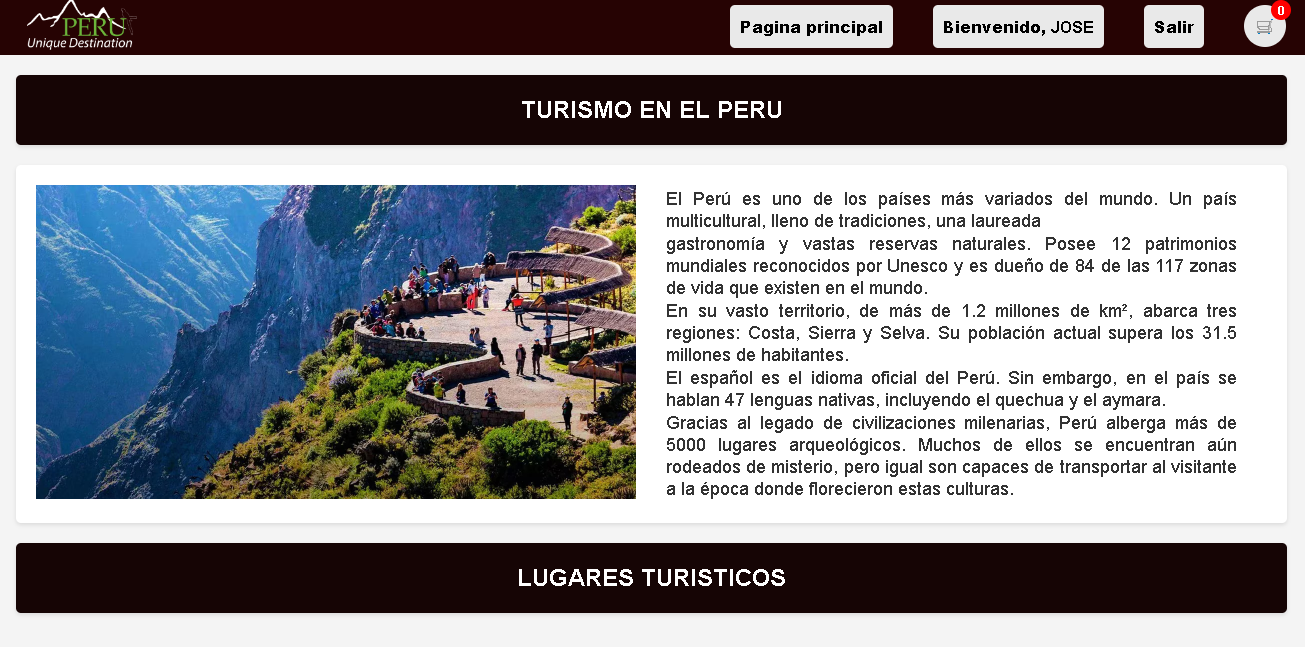
\includegraphics[width=16cm]{img/PAGINA INICIAL 1.png}
        \newline\newline
        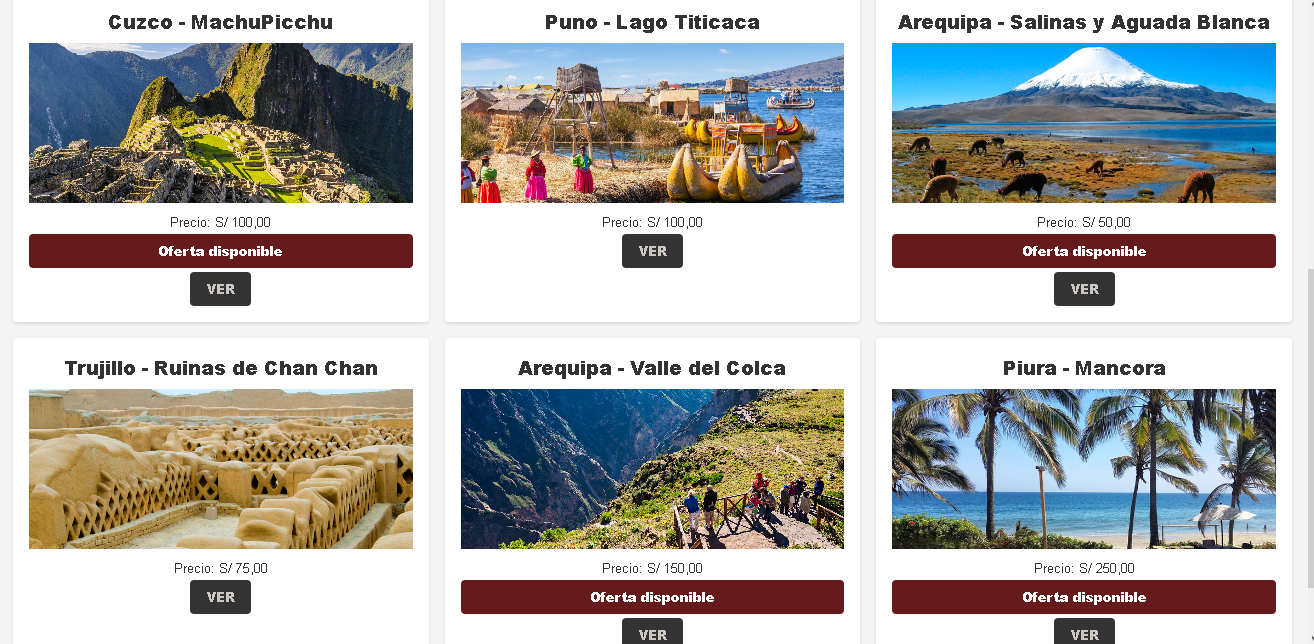
\includegraphics[width=16cm]{img/imagen_2023-06-29_011451598.png}
        Esa fue la pantalla, pero que tenia a un usuario ya logeado, por lo que al hacer click en salir se nos dara la opcion de registrarnos o logearnos de nuevo:
        \newline\newline
        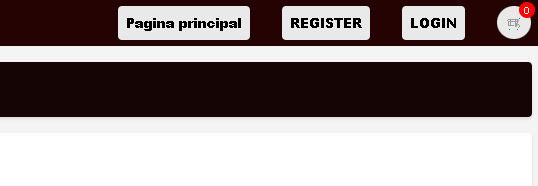
\includegraphics[width=16cm]{img/deslog.png}
        \newline\newline\newline
        Ahora veamos lo que nos aparece haciendo click en "VER" de un destino es especifico:
        \newline
        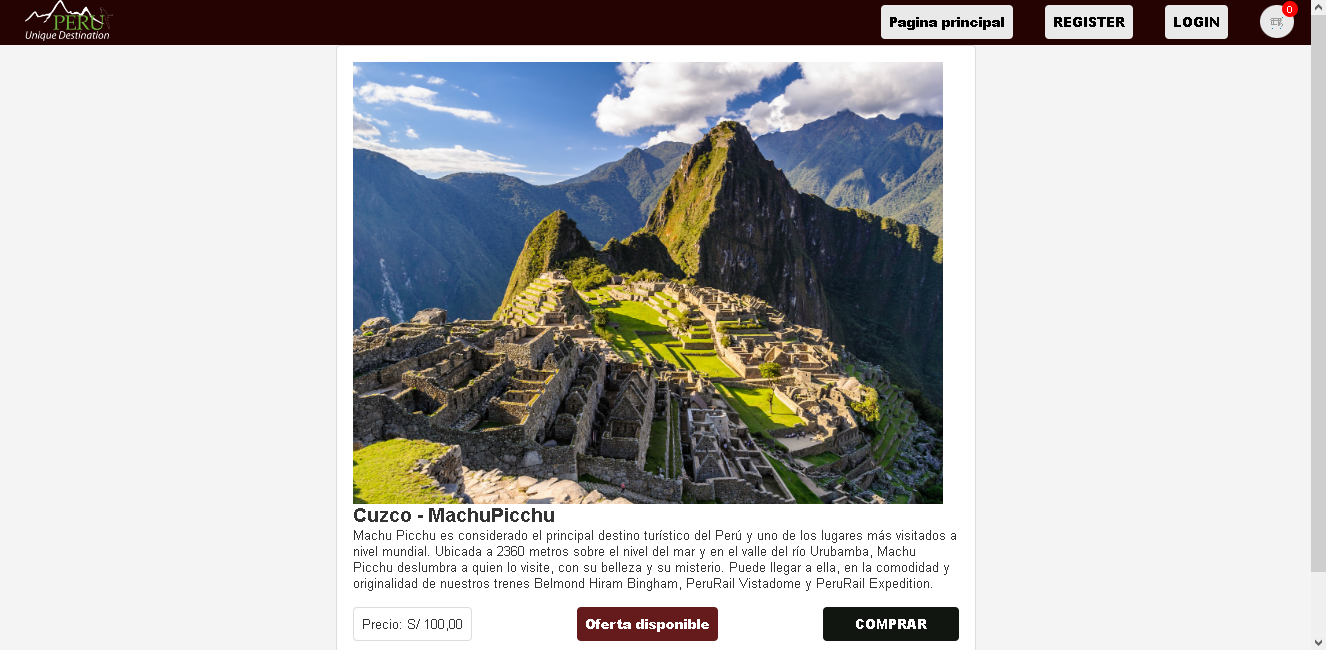
\includegraphics[width=16cm]{img/vistaDestinoEspecifico.png}
        Como vemos se nos muestra el destino con sus respectivos atributos, siguiendo el modelo creado\newline

        Ahora veamos el apartado de registro, en donde se nos pedira llenar un forms simple:\newline
        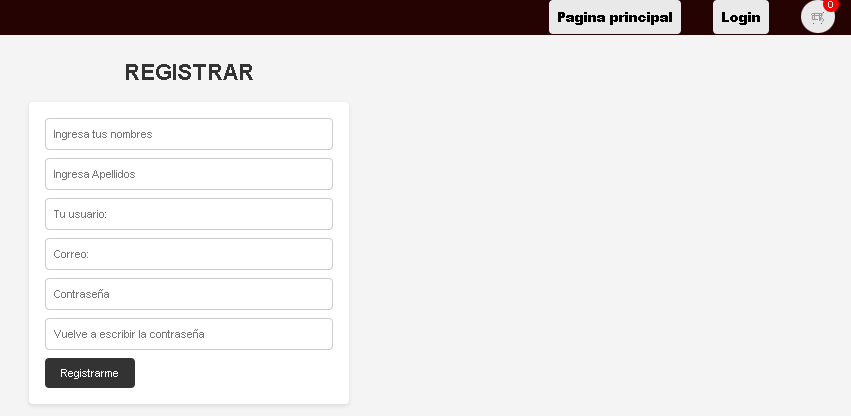
\includegraphics[width=16cm]{img/REGISTRO.png}
        \newline
        Por otra parte esta el apartado de logeo, donde accederemos a un usuario ya existente\newline
        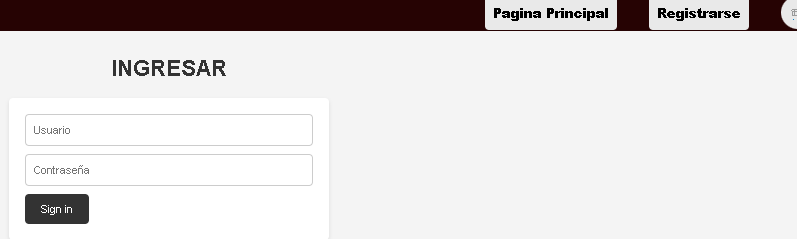
\includegraphics[width=16cm]{img/LOGIN.png}
        \newline
        Por ultimo revisemos usuarios y los destinos guardados en la pagina de administracion:\newline
         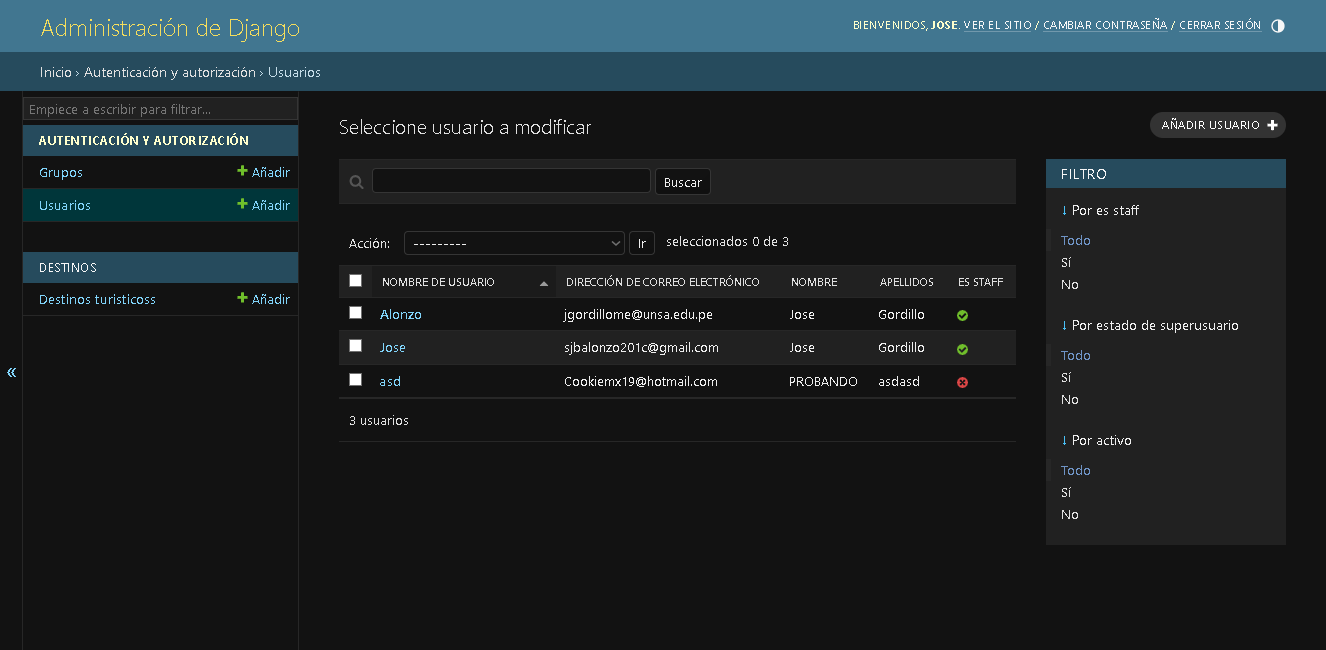
\includegraphics[width=16cm]{img/usuarios.png}
          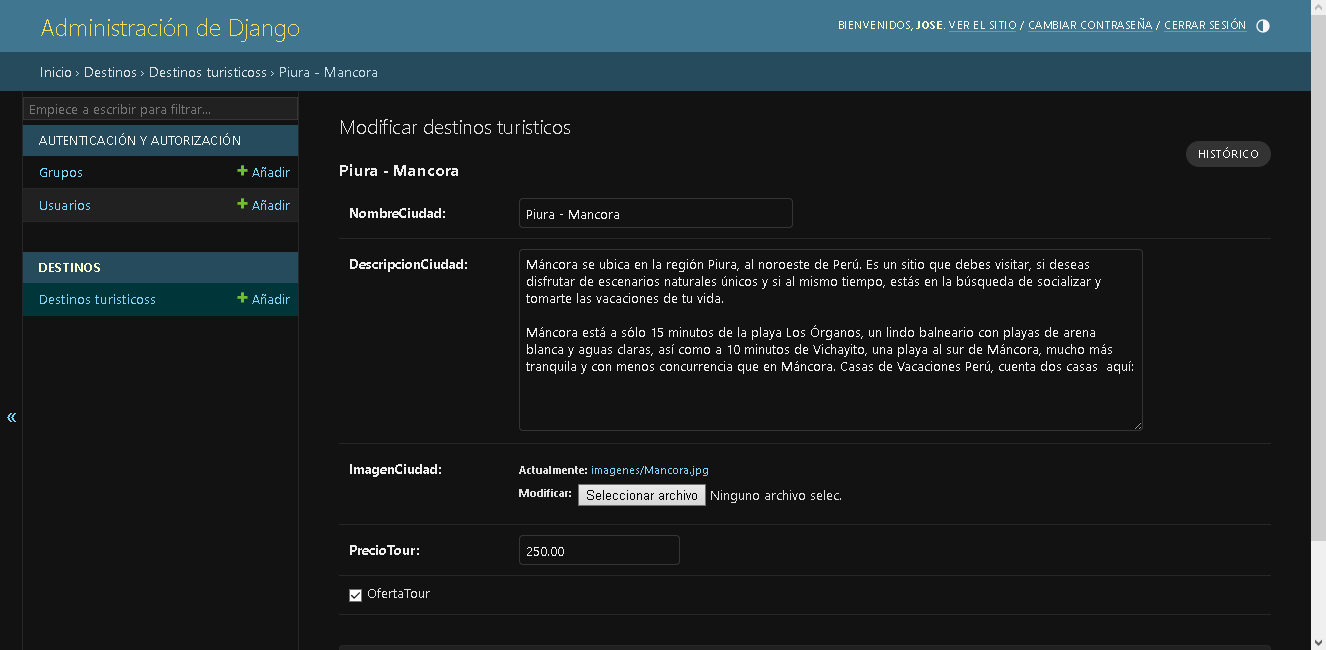
\includegraphics[width=16cm]{img/EJEMPLOdestino.png}
        Link donde esta alojado el video (FlipGrid):\newline
        GRUPO:
        \url{https://flip.com/groups/14644257/topics/36969916/responses}\newline
        VIDEO ESPECIFICO:
        \url{https://flip.com/s/rYjXvXLaSCPu}
        
\section{Cuestionario}
	- Sin cuestionario -	
 \newpage
 \section{Conclusiones}
	\begin{itemize}
		\item El desarrollo de aplicaciones utilizando Django ofrece una combinación de productividad, escalabilidad, seguridad y flexibilidad. Su enfoque basado en convenciones, su sólida arquitectura y su amplia comunidad de desarrolladores hacen de Django una opción poderosa para crear aplicaciones web de calidad..
            \item El uso de tags en Django mejora la flexibilidad, la legibilidad y la modularidad de las plantillas HTML, permitiendo la generación de contenido dinámico y la separación clara entre la lógica del backend y la presentación visual. Esto contribuye a un desarrollo más eficiente y estructurado de aplicaciones web utilizando el framework Django.
            \item El uso de plantillas y archivos estáticos en Django ofrece flexibilidad, reutilización de código, separación de la lógica y la presentación, y un rendimiento eficiente en la entrega de recursos estáticos. Estas características hacen que el desarrollo y mantenimiento de aplicaciones web sea más organizado, escalable y fácil de mantener.
            \item Las vistas en Django son componentes clave para controlar la lógica del backend en una aplicación web. Permiten la separación de responsabilidades, interactúan con modelos y bases de datos, generan respuestas personalizadas y pueden ser probadas para garantizar un correcto funcionamiento. Su uso adecuado contribuye a un desarrollo eficiente, escalable y mantenible de aplicaciones web utilizando el framework Django.
	\end{itemize}	
\clearpage

\section{Referencias}
\begin{itemize}	
    \item \url{https://www.w3schools.com/python/python_reference.asp}
    \item \url{ https://docs.python.org/3/tutorial/}
    \item \url{https://docs.djangoproject.com/en/4.0/}
    \item \url{https://www.youtube.com/watch?v=M4NIs4BM1dk}
    \item \url{https://pip.pypa.io/en/latest/user_guide/}
    \item \url{https://www.youtube.com/watch?v=OTmQOjsl0eg}
\end{itemize}	
	
%\clearpage
%\bibliographystyle{apalike}
%\bibliographystyle{IEEEtranN}
%\bibliography{bibliography}
			
\end{document}